% Options for packages loaded elsewhere
\PassOptionsToPackage{unicode}{hyperref}
\PassOptionsToPackage{hyphens}{url}
\PassOptionsToPackage{dvipsnames,svgnames*,x11names*}{xcolor}
%
\documentclass[
]{article}
\usepackage{lmodern}
\usepackage{amssymb,amsmath}
\usepackage{ifxetex,ifluatex}
\ifnum 0\ifxetex 1\fi\ifluatex 1\fi=0 % if pdftex
  \usepackage[T1]{fontenc}
  \usepackage[utf8]{inputenc}
  \usepackage{textcomp} % provide euro and other symbols
\else % if luatex or xetex
  \usepackage{unicode-math}
  \defaultfontfeatures{Scale=MatchLowercase}
  \defaultfontfeatures[\rmfamily]{Ligatures=TeX,Scale=1}
\fi
% Use upquote if available, for straight quotes in verbatim environments
\IfFileExists{upquote.sty}{\usepackage{upquote}}{}
\IfFileExists{microtype.sty}{% use microtype if available
  \usepackage[]{microtype}
  \UseMicrotypeSet[protrusion]{basicmath} % disable protrusion for tt fonts
}{}
\makeatletter
\@ifundefined{KOMAClassName}{% if non-KOMA class
  \IfFileExists{parskip.sty}{%
    \usepackage{parskip}
  }{% else
    \setlength{\parindent}{0pt}
    \setlength{\parskip}{6pt plus 2pt minus 1pt}}
}{% if KOMA class
  \KOMAoptions{parskip=half}}
\makeatother
\usepackage{xcolor}
\IfFileExists{xurl.sty}{\usepackage{xurl}}{} % add URL line breaks if available
\IfFileExists{bookmark.sty}{\usepackage{bookmark}}{\usepackage{hyperref}}
\hypersetup{
  colorlinks=true,
  linkcolor=blue,
  filecolor=Maroon,
  citecolor=Blue,
  urlcolor=Blue,
  pdfcreator={LaTeX via pandoc}}
\urlstyle{same} % disable monospaced font for URLs
\usepackage{listings}
\newcommand{\passthrough}[1]{#1}
\lstset{defaultdialect=[5.3]Lua}
\lstset{defaultdialect=[x86masm]Assembler}
\usepackage{longtable,booktabs}
% Correct order of tables after \paragraph or \subparagraph
\usepackage{etoolbox}
\makeatletter
\patchcmd\longtable{\par}{\if@noskipsec\mbox{}\fi\par}{}{}
\makeatother
% Allow footnotes in longtable head/foot
\IfFileExists{footnotehyper.sty}{\usepackage{footnotehyper}}{\usepackage{footnote}}
\makesavenoteenv{longtable}
\usepackage{graphicx}
\makeatletter
\def\maxwidth{\ifdim\Gin@nat@width>\linewidth\linewidth\else\Gin@nat@width\fi}
\def\maxheight{\ifdim\Gin@nat@height>\textheight\textheight\else\Gin@nat@height\fi}
\makeatother
% Scale images if necessary, so that they will not overflow the page
% margins by default, and it is still possible to overwrite the defaults
% using explicit options in \includegraphics[width, height, ...]{}
\setkeys{Gin}{width=\maxwidth,height=\maxheight,keepaspectratio}
% Set default figure placement to htbp
\makeatletter
\def\fps@figure{htbp}
\makeatother
\setlength{\emergencystretch}{3em} % prevent overfull lines
\providecommand{\tightlist}{%
  \setlength{\itemsep}{0pt}\setlength{\parskip}{0pt}}
\setcounter{secnumdepth}{5}


%% pandoc-tablenos: required package
\usepackage{cleveref}

%% pandoc-eqnos: disable brackets around cleveref numbers
\creflabelformat{equation}{#2#1#3}
\ifluatex
  \usepackage{selnolig}  % disable illegal ligatures
\fi
\newlength{\cslhangindent}
\setlength{\cslhangindent}{1.5em}
\newlength{\csllabelwidth}
\setlength{\csllabelwidth}{3em}
\newenvironment{CSLReferences}[3] % #1 hanging-ident, #2 entry sp
 {% don't indent paragraphs
  \setlength{\parindent}{0pt}
  % turn on hanging indent if param 1 is 1
  \ifodd #1 \everypar{\setlength{\hangindent}{\cslhangindent}}\ignorespaces\fi
  % set line spacing
  % set entry spacing
  \ifnum #2 > 0
  \setlength{\parskip}{#3\baselineskip}
  \fi
 }%
 {}
\usepackage{calc} % for \widthof, \maxof
\newcommand{\CSLBlock}[1]{#1\hfill\break}
\newcommand{\CSLLeftMargin}[1]{\parbox[t]{\maxof{\widthof{#1}}{\csllabelwidth}}{#1}}
\newcommand{\CSLRightInline}[1]{\parbox[t]{\linewidth}{#1}}
\newcommand{\CSLIndent}[1]{\hspace{\cslhangindent}#1}

\author{}
\date{}

\begin{document}

\lstset{columns=fullflexible,breaklines=true,basicstyle=\small\ttfamily,backgroundcolor=\color{gray!10}}

\hypertarget{the-naive-bayes-classification-method}{%
\section{The Naive Bayes classification
method}\label{the-naive-bayes-classification-method}}

\hypertarget{introduction}{%
\subsection{Introduction}\label{introduction}}

In our discussion of Bayes Theorem, we looked at a situation in which we
had a population consisting of people infected with COVID-19 and people
not infected, and we had a test that we could apply to determine which
class an individual belonged to. Because our test was not 100 percent
reliable, a positive test result didn't guarantee that a person was
infected, and we used Bayes Theorem to evaluate how to interpret the
positive test result. More specifically, our information about the test
performance gave us the the conditional probabilities of positive and
negative test results given infection status -- so for example we were
given \(P(+|\mathrm{infected})\), the chance of getting a positive test
assuming the person is infected -- and we used Bayes Theorem to
determine \(P(\mathrm{infected}|+)\), the chance that a person was
infected given a positive test result.

The Naive Bayes classification method is a generalization of this idea.
We have data that belongs to one of two classes, and based on the
results of a series of tests, we wish to decide which class a particular
data point belongs to. For one example, we are given a collection of
product reviews from a website and we wish to classify those reviews as
either ``positive'' or ``negative.'' This type of problem is called
``sentiment analysis.'' For another, related example, we have a
collection of emails or text messages and we wish to label those that
are likely ``spam'' emails. In both of these examples, the ``test'' that
we will apply is to look for the appearance or absence of certain key
words that make the text more or less likely to belong to a certain
class. For example, we might find that a movie review that contains the
word ``great'' is more likely to be positive than negative, while a
review that contains the word ``boring'' is more likely to be negative.

The reason for the word ``naive'' in the name of this method is that we
will derive our probabilities from empirical data, rather than from any
deeper theory. For example, to find the probability that a negative
movie review contains the word ``boring,'' we will look at a bunch of
reviews that our experts have said are negative, and compute the
proportion of those that contain the word boring. Indeed, to develop our
family of tests, we will rely on a training set of already classified
data from which we can determine estimates of probabilities that we
need.

\hypertarget{an-example-dataset}{%
\subsection{An example dataset}\label{an-example-dataset}}

To illustrate the Naive Bayes algorithm, we will work with the
``Sentiment Labelled Sentences Data Set''
({[}\protect\hyperlink{ref-sentences}{1}{]}). This dataset contains 3
files, each containing 1000 documents labelled \(0\) or \(1\) for
``negative'' or ``positive'' sentiment. There are 500 of each type of
document in each file. One file contains reviews of products from
amazon.com; one contains yelp restaurant reviews, and one contains movie
reviews from imdb.com.

Let's focus on the amazon reviews data. Here are some samples:

\begin{lstlisting}
So there is no way for me to plug it in here in the US unless I go by a converter.  0
Good case, Excellent value. 1
Great for the jawbone.  1
Tied to charger for conversations lasting more than 45 minutes.MAJOR PROBLEMS!! 0
The mic is great.   1
I have to jiggle the plug to get it to line up right to get decent volume.  0
If you have several dozen or several hundred contacts, then imagine the fun of sending each of them one by one. 0
If you are Razr owner...you must have this! 1
Needless to say, I wasted my money. 0
What a waste of money and time!.    0
\end{lstlisting}

As you can see, each line consists of a product review followed by a
\(0\) or \(1\); in this file the review is separated from the text by a
tab character.

\hypertarget{bernoulli-tests}{%
\subsection{Bernoulli tests}\label{bernoulli-tests}}

We will describe the ``Bernoulli'' version of a Naive Bayes classifier
for this data. The building block of this method is a test based on a
single word. For example, let's consider the word \textbf{great} among
all of our amazon reviews. It turns out that \textbf{great} occurs \(5\)
times in negative reviews and \(92\) times in positive reviews among our
\(1000\) examples. So it seems that seeing the word \textbf{great} in a
review makes it more likely to be positive. The appearances of great are
summarized in \cref{tbl:great} . We write
\textasciitilde{}\textbf{great} for the case where \textbf{great} does
\emph{not} appear.

\begin{longtable}[]{@{}llll@{}}
\caption{Ocurrences of \textbf{great} by type of review
.\label{tbl:great}}\tabularnewline
\toprule
& + & - & total\tabularnewline
\midrule
\endfirsthead
\toprule
& + & - & total\tabularnewline
\midrule
\endhead
\textbf{great} & 92 & 5 & 97\tabularnewline
\textasciitilde{}\textbf{great} & 408 & 495 & 903\tabularnewline
total & 500 & 500 & 1000\tabularnewline
\bottomrule
\end{longtable}

In this data, positive and negative reviews are equally likely so
\(P(+)=P(-)=.5\) From this table, and Bayes Theorem, we obtain the
empirical probabilities (or ``naive'' probabilities).

\[
P(\mathbf{great} | +) = \frac{92}{500} = .184
\]

and

\[
P(\mathbf{great}) = \frac{97}{1000} = .097
\]

Therefore

\[
P(+|\mathbf{great}) = \frac{.184}{.097}(.5) = 0.948.
\]

In other words, \emph{if} you see the word \textbf{great} in a review,
there's a 95\% chance that the review is positive.

What if you \emph{do not} see the word \textbf{great}? A similar
calculation from the table yields

\[
P(+|\sim\mathbf{great}) = \frac{408}{903} = .452
\]

In other words, \emph{not} seeing the word great gives a little evidence
that the review is negative (there's a 55\% chance it's negative) but
it's not that conclusive.

The word \textbf{waste} is associated with negative reviews. It's
statistics are summarized in \cref{tbl:waste}.

\begin{longtable}[]{@{}llll@{}}
\caption{Ocurrences of \textbf{waste} by type of review
.\label{tbl:waste}}\tabularnewline
\toprule
& + & - & total\tabularnewline
\midrule
\endfirsthead
\toprule
& + & - & total\tabularnewline
\midrule
\endhead
\textbf{waste} & 0 & 14 & 14\tabularnewline
\textasciitilde{}\textbf{waste} & 500 & 486 & 986\tabularnewline
total & 500 & 500 & 1000\tabularnewline
\bottomrule
\end{longtable}

Based on this data, the ``naive'' probabilities we are interested in
are:

\begin{align*}
P(+|\mathbf{waste}) &= 0\\
P(+|\sim\mathbf{waste}) &= .51
\end{align*}

In other words, if you see \textbf{waste} you definitely have a negative
review, but if you don't, you're only slightly more likely to have a
positive one.

What about combining these two tests? Or using even more words? We could
analyze our data to count cases in which both \textbf{great} and
\textbf{waste} occur, in which only one occurs, or in which neither
occurs, within the two different categories of reviews, and then use
those counts to estimate empirical probabilities of the joint events.
But while this might be feasible with two words, if we want to use many
words, the number of combinations quickly becomes huge. So instead, we
make a basic, and probably false, assumption, but one that makes a
simple analysis possible.

\textbf{Assumption:} We assume that the presence or absence of the words
\textbf{great} and \textbf{waste} in a particular review (positive or
negative) are independent events. More generally, given a collection of
words \(w_1,\ldots, w_k\), we assume that their occurences in a given
review are independent events.

Independence means that we have \begin{align*}
P(\mathbf{great},\mathbf{waste}|\pm) &= P(\mathbf{great}|\pm)P(\mathbf{waste}|\pm)\\
P(\mathbf{great},\sim\mathbf{waste}|\pm) &= P(\mathbf{great}|\pm)P(\sim\mathbf{waste}|\pm)\\
 &\vdots \\
\end{align*}

So for example, if a document contains the word \textbf{great} and does
\emph{not} contain the word \textbf{waste}, then the probability of it
being a positive review is: \[
P(+|\mathbf{great},\sim\mathbf{waste}) = \frac{P(\mathbf{great}|+)P(\sim\mathbf{waste}|+)P(+)}{P(\mathbf{great},\sim\mathbf{waste})}
\] while the probability of it being a negative review is \[
P(-|\mathbf{great},\sim\mathbf{waste}) = \frac{P(\mathbf{great}|-)P(\sim\mathbf{waste}|-)P(-)}{P(\mathbf{great},\sim\mathbf{waste})}
\] Rather than compute these probabilities (which involves working out
the denominators), let's just compare them. Since they have the same
denominators, we just need to compare numerators, which we call \(L\)
for likelihood: Using the data from \cref{tbl:great} and
\cref{tbl:waste}, we obtain: \[
L(+|\mathbf{great},\sim\mathbf{waste}) = (.184)(1)(.5) = .092
\] and \[
L(-|\mathbf{great},\sim\mathbf{waste}) = (.01)(.028)(.5) = .00014
\] so our data suggests strongly that this is a positive review.

\hypertarget{feature-vectors}{%
\subsection{Feature vectors}\label{feature-vectors}}

To generalize this, suppose that we have extracted keywords
\(w_1,\ldots, w_k\) from our data and we have computed the empirical
values \(P(w_{i}|+)\) and \(P(w_{i}|-)\) by counting the fraction of
positive and negative reviews that contain the word \(w_{i}\):

\[
P(w_{i}|\pm) = \frac{\hbox{\rm number of $\pm$ reviews that mention $w_{i}$}}{\hbox{\rm number of $\pm$ reviews total}}
\]

Notice that we only count \emph{reviews}, not \emph{ocurrences}, so that
if a word occurs multiple times in a review it only contributes 1 to the
count. That's why this is called the \emph{Bernoulli} Naive Bayes -- we
are thinking of each keyword as yielding a yes/no test on each review.

Given a review, we look to see whether each of our \(k\) keywords
appears or does not. We encode this information as a vector of length
\(k\) containing \(0\)'s and \(1\)'s indicating the absence or presence
of the \(k\)th keyword. Let's call this vector the \emph{feature vector}
for the review.

For example, if our keywords are \(w_1=\mathbf{waste}\),
\(w_2=\mathbf{great}\), and \(w_3=\mathbf{useless}\), and our review
says

\begin{lstlisting}
This phone is useless, useless, useless!  What a waste!
\end{lstlisting}

then the associated feature vector is \(f=(1,0,1)\).

For the purposes of classification of our reviews, we are going to
forget entirely about the text of our reviews and work only with the
feature vectors. From an abstract perspective, then, by choosing our
\(k\) keywords, our ``training set'' of \(N\) labelled reviews can be
replaced by an \(N\times k\) matrix \(X=(x_{ij})\) with entries \(0\) or
\(1\), where \(x_{ij}=1\) if and only if the \(j^{th}\) keyword appears
in the \(i^{th}\) review.

The labels of \(0\) or \(1\) for unfavorable or favorable reviews can
also be packaged up into a \(N\times 1\) vector \(Y\) that serves as our
``target'' variable.

Setting things up this way lets us express the computations of our
probabilities \(P(w_{i}|\pm)\) in vector form. In fact,
\(Y^{\intercal}X\) is the sum of the rows of \(X\) corresponding to
positive reviews, and therefore, letting \(N_{\pm}\) denote the number
of \(\pm\) reviews, \[
P_{+} = \frac{1}{N_{+}}Y^{\intercal}X = \left[\begin{array}{cccc} P(w_{1}|+)& P(w_{2}|+) & \cdots &P(w_{k}|+)\end{array}\right].
\] Similarly, since \(Y\) and \(X\) have zero and one entries only, if
we write \(1-Y\) and \(1-X\) for the matrices obtained by replacing
every entry \(z\) by \(1-z\) in each matrix, we have: \[
P_{-} = \frac{1}{N_{-}}(1-Y)^{\intercal}X =  \left[\begin{array}{cccc} P(w_{1}|-)& P(w_{2}|-) & \cdots &P(w_{k}|-)\end{array}\right].
\]

Note that the number of positive reviews is \(N_{+}=Y^{\intercal}Y\) and
the number of negative ones is \(N_{-}=N-N_{+}\). Since \(P(+)\) is the
fraction of positive reviews among all reviews, we can compute it as
\(P(+)=\frac{1}{N}Y^{\intercal}Y\), and \(P(-)=1-P(+)\).

\hypertarget{likelihood}{%
\subsection{Likelihood}\label{likelihood}}

If a review has an associated feature vector \(f=(f_1,\ldots, f_k)\),
then by independence the probability of that feature vector ocurring
within one of the \(\pm\) classes is \[
P(f|\pm) = \prod_{i: f_{i}=1} P(w_{i}|\pm)\prod_{i: f_{i}=0}(1-P(w_{i}|\pm))
\] which we can also write \begin{equation}
P(f|\pm) = \prod_{i=1}^{k} P(w_{i}|\pm)^{f_{i}}(1-P(w_{i}|\pm))^{(1-f_{i})}.
\label{eq:likelihood}\end{equation}

These products aren't practical to work with -- they are often the
product of many, many small numbers and are therefore really tiny.
Therefore it's much more practical to work with their logarithms.
\begin{equation}
\log P(f|\pm) = \sum_{i=1}^{k} f_{i}\log P(w_{i}|\pm) + (1-f_{i})\log(1-P(w_{i}|\pm))
\label{eq:loglikelihood}\end{equation}

If we have a group of reviews \(N\) organized in a matrix \(X\), where
each row is the feature vector associated to the corresponding review,
then we can compute all of this at once. We'll write
\(\log P_{\pm}=\log P(X|\pm)\) as the row vector whose \(i^{th}\) entry
is \(\log P(f_{i}|\pm)\):

\begin{equation}
\log P(X|\pm) = X(\log P_{\pm})^{\intercal}+(1-X)(\log (1-P_{\pm}))^{\intercal}.
\label{eq:matrixlikelihood}\end{equation}

By Bayes Theorem, we can express the chance that our review with feature
vector \(f\) is positive or negative by the formula: \[
\log P(\pm|f) = \log P(f|\pm)+\log P(\pm) - \log P(f)
\] where \[
P(\pm) = \frac{\hbox{\rm the number of $\pm$ reviews}}{\hbox{\rm total number of reviews}}
\] and \(P(f)\) is the fraction of reviews with the given feature
vector. (Note: in practice, some of these probabilities will be zero,
and so the log will not be defined. A common practical approach to
dealing with this is to introduce a ``fake document'' into both classes
in which every vocabulary word appears -- this guarantees that the
frequency matrix will have no zeros in it).

A natural classification rule would be to say that a review is positive
if \(\log P(+|f)>\log P(-|f)\), and negative otherwise. In applying
this, we can avoid computing \(P(f)\) by just comparing
\(\log P(f|+)+\log P(+)\) and \(\log P(f|-)+\log P(-)\) computed using
\cref{eq:loglikelihood}. Then we say:

\begin{itemize}
\tightlist
\item
  a review is positive if
  \(\log P(f|+)+\log P(+)>\log P(f|-)+\log P(-)\) and negative
  otherwise.
\end{itemize}

Again we can exploit the matrix structure to do this for a bunch of
reviews at once. Using \cref{eq:matrixlikelihood} and the vectors
\(P_{\pm}\) we can compute column vectors corresponding to both sides of
our decision inequality and subtract them. The positive entries indicate
positive reviews, and the negative ones, negative reviews.

\hypertarget{other-applications}{%
\subsection{Other applications}\label{other-applications}}

We developed the Naive Bayes method for sentiment analysis, but once we
chose a set of keywords our training data was reduced to an
\(N\times k\) matrix \(X\) of \(0/1\) entries, together with an
\(N\times 1\) target column vector \(Y\). Then our classification
problem is to decide whether a given vector of \(k\) entries, all \(0\)
or \(1\), is more likely to carry a \(0\) or \(1\) label. All of the
parameters we needed for Naive Bayes -- the various probabilities -- can
be extracted from the matrix \(X\).

For example, suppose we have a collection of images represented as
black/white pixels in a grid that belong to one of two classes. For
example, we might have \(28x28\) bitmaps of handwritten zeros and ones
that are labelled, and we wish to construct a classifier that can decide
whether a new \(28x28\) bitmap is a zero or one. An example of such a
bitmap is given in \cref{fig:mnist0}. We can view each \(28x28\) bitmap
as a vector of length \(784\) with \(0/1\) entries and apply the same
approach outlined above.

\begin{figure}
\hypertarget{fig:mnist0}{%
\centering
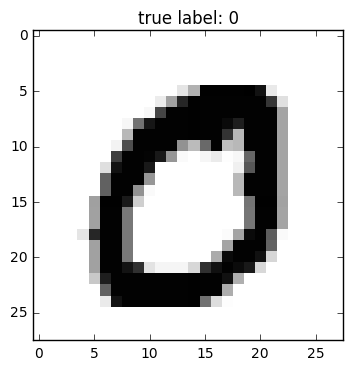
\includegraphics[width=2in,height=\textheight]{../img/mnist_data_10_0.png}
\caption{Handwritten 0}\label{fig:mnist0}
}
\end{figure}

\hypertarget{other-models-the-binomial-and-gaussian-models.}{%
\subsection{Other models: the binomial and gaussian
models.}\label{other-models-the-binomial-and-gaussian-models.}}

We have discussed a version of Naive Bayes based on the Bernoulli model,
in which we imagine applying a set of independent yes/no tests to some
data to determine its most likely class. Concretely, in our sentiment
analysis problem, we looked for the presence or absence of certain
words, but paid no attention to whether a word occurred more than once.

The binomial model is an alternative approach to the Bernoulli model and
takes a different point of view on the text data. It is sometimes called
the ``bag of words'' model. Suppose I have a vocabulary of words \(w\),
and two types of documents \(\pm\). For each word we have probabilities
\(P_{+}(w)\) and \(P_{-}(w)\) that measure the chance that a particular
word in each class is the given word. These probabilities can be derived
in a naive sense by looking at the frequency with which they occur in
documents of the two classes. In this statistical model a document in
class \(+\) is constructed by successively choosing words from the
vocabulary according to the probabilities \(P_{+}(w)\).

Given a document to classify, one looks at the frequencies of the
vocabulary words and computes the likelihood of that distribution in
each of the two classes, and chooses the more likely class.

This approach is better suited to longer documents, and it requires
working with large vocabularies, but it does take account of how often
the vocabulary words appear in the document.

The Gaussian model takes a different approach and is useful for
classifying numerical data. Given a set of labelled training data, one
assumes that each feature comes from a normal distribution, with the
mean and variance depending on the associated class. One uses the
training data to estimate these means and variances. Then, given a piece
of data to classify, one computes the likelihood of the data arising
from the two different classes, and chooses the more likely one.

What unites all of these methods under the heading of Naive Bayes is
that the parameters are estimated simply from empirical data -- that's
the naive part -- and Bayes theorem is used to compute the likelihood of
membership in each of the two classes.

\hypertarget{bibliography}{%
\section*{References}\label{bibliography}}
\addcontentsline{toc}{section}{References}

\hypertarget{refs}{}
\begin{CSLReferences}{0}{0}
\leavevmode\hypertarget{ref-sentences}{}%
\CSLLeftMargin{{[}1{]} }
\CSLRightInline{\textsc{U.C. Irvine ML Repository}. {Sentiment Labelled
Sentences Data Set}.Available at
\url{https://archive.ics.uci.edu/ml/datasets/Sentiment+Labelled+Sentences}.}

\end{CSLReferences}

\end{document}
